\section{Evaluierung der Modelle}\raggedbottom
\label{evalmetric}
Nachfolgend werden die in dieser Arbeit konstruierten Modelle evaluiert.
Die unterschiedlichen Optimierungen der Latentvektoren für ein Optimus Modell und des Cellstates für \textsc{BiMeanVAE} werden auf dem Amazon und dem Yelp Datensatz verglichen und mit dem aktuellem State-of-the-Art Modell COOP in Relation gesetzt.
Es existieren im Dev-Datensatz und Test-Datensatz jeweils 8 Eingabebewertungen und beim Amazon Datensatz drei Gold-Summaries, beim Yelp Datensatz eine Gold-Summary zum Evaluieren der generierten Ausgabebewertungen.
Die Eingabebewertungen werden durch ein Optimus VAE Modell und ein \textsc{BiMeanVAE} Modell in Latentvektoren umgewandelt.
Anschließend werden, mittels der in Abschnitt \ref{coop_chap} dargestellter COOP Herangehensweise, die Latentvektoren kombiniert, um den \textit{Input-Output-Overlap} zu maximieren. 
Die Latentvektoren werden mittels in dieser Arbeit eingeführtem Attribut-Modell optimiert, um detailreiche und umfassende Durchschnittsrezensionen zu erhalten.

\subsection{Evaluationsmetriken}
\label{eval_metrics_chapter}
Die generierten Textbewertungen werden mit den drei Gold-Summaries verglichen.
Zum Vergleich der generierten Rezensionen wird die ROUGE (\textbf{R}ecall-\textbf{O}riented \textbf{U}nderstudy for \textbf{G}isting \textbf{E}valuation)-Metrik verwendet \citep{lin-2004-rouge}.
Die ROUGE-N Metrik misst die Anzahl der übereinstimmenden N-Grams zwischen dem generierten Text und den Referenztexten. 
Ein N-Gram ist eine N-lange sequentielle Folge von Wörtern innerhalb der Texte. 

Zur Bewertung der generierten Rezensionen werden die vorhergesagten Ergebnisse mit den korrekten Ergebnissen verglichen. 
Die Konfusionsmatrix in Abbildung \ref{confusionmatrix} ist eine Wahrheitsmatrix, welche die Einteilung der vorhergesagten Ergebnisse ermöglicht. 
True Positive (TP) und True Negative (TN) sind von dem Modell korrekt vorhergesagte Ergebnisse, False Positive (FP) und False Negative (FN) ist eine Klasse von falsch vorhergesagten Ergebnissen.



\begin{figure}[h!]
    \centering
\begin{tikzpicture}[
    box/.style={draw,rectangle,minimum size=2cm,text width=1.5cm,align=left}]
    \matrix (conmat) [row sep=.1cm,column sep=.1cm] {
    \node (tpos) [box,
        label=left:Positive,
        label=above:Positive,
        ] {True \\ positive};
    &
    \node (fneg) [box,
        label=above:Negative] {False \\ negative};
    \\
    \node (fpos) [box,
        label=left:Negative] {False \\ positive};
    &
    \node (tneg) [box] {True \\ negative};
    \\
    };
    \node [left=.05cm of conmat,text width=1.5cm,align=right] {\textbf{Referenz}};
    \node [above=.05cm of conmat] {\textbf{Vorhersage}};
\end{tikzpicture}
\caption{Konfusionsmatrix zur Berechnung des ROUGE-N Scores}
\label{confusionmatrix}
\end{figure}

Zur Berechnung des ROUGE-N Scores werden die einzelnen Textabschnitte in eine Menge aus N-Grams zerlegt.
Mittels der Konfusionsmatrix in Abbildung \ref{confusionmatrix} lassen sich Precision (P) und Recall (R) definieren:
\begin{addmargin}[30pt]{30pt}
    \textbf{Precision}: 
    Der Precision Wert ergibt sich aus dem Verhältnis der korrekt vorhergesagten N-Grams und der Anzahl der insgesamt vorhergesagten N-Grams.
    \begin{align*}
    \text{P} = \frac{\text{TP}}{\text{TP}+\text{FP}}
    \end{align*}

    \textbf{Recall}:
    Recall ist als Verhältnis zwischen den korrekt vorhergesagten N-Grams und den N-Grams aus der Referenz definiert.
    \begin{align*}
    \text{R} = \frac{\text{TP}}{\text{TP}+\text{FN}}
    \end{align*}

    $\textbf{F}_\textbf{1}$:
    Das F1-Maß beschreibt das harmonische Mittel zwischen Precision und Recall.
    \begin{align*}
    \text{F}_\text{1} = \frac{2\text{PR}}{\text{P}+\text{R}}
    \end{align*}
\end{addmargin}

In der Evaluation werden die ROUGE-1, ROUGE-2 und ROUGE-L Werte miteinander verglichen.
ROUGE-1 verwendet als N-Gram Unigramme, ROUGE-2 Bigramme und ROUGE-L misst die längste gleiche Subsequenz zwischen Vorhersage und Referenz.

Da die ROUGE-Scores lediglich die einzelnen Wortsequenzen miteinander vergleichen, findet die semantische Bedeutung und Ähnlichkeit der Bewertungen mit der Referenz keinen Einfluss.
Hier erzielen zum Beispiel Synonyme keine guten ROUGE-Scores, obwohl sie eine semantische Übereinstimmung haben.
Um trotzdem die semantische Ähnlichkeit zwischen Bewertungen und Referenz zu messen, wird als weitere Metrik der Moverscore aus Abschnitt \ref{moverscore} verwendet.
Der Moverscore basiert auf BERT und vergleicht Context-Embeddings mittels Earth-Mover-Distance \citep{emd}. Als Metrik konnte der Moverscore hohe Korrelationen mit menschlichem Urteilsvermögen aufweisen.


\subsection{Moverscore}
\label{moverscore}
Der Moverscore \citep{moverscore_paper} ist eine Evaluationsmetrik, die semantische Inhalte zwischen zwei Textsequenzen vergleicht und diesen einen Ähnlichkeitswert zuweist.
Das Ziel vom Moverscore ist es, eine Metrik abzubilden, die sich einer menschlichen Bewertung der Ähnlichkeit von zwei Sequenzen annähert. 
Im Gegensatz zu anderen Textähnlichkeitsmetriken, die lediglich die Überlappungen von Tokens innerhalb der Sequenzen messen, ohne die Semantik der Wörter zu bewerten, 
bildet sich der Moverscore aus einer Kombination bestehend aus einer im Kontext eingebetteten Repräsentation der einzelnen Textsequenzen, die eine semantische Distanz untereinander abbilden.
Die semantische Distanz wird über die Word Mover Distance \citep{wordmoverdistance}, einer Metrik basierend auf der Earth Mover Distance, bestimmt. Es wird ein minimaler Transportfluss zwischen den einzelnen Sequenzen errechnet.
Die Worteinbettungen werden durch ein BERT Modell erzeugt.

Insgesamt ist der Moverscore für die Bewertungsgenerierung ein wichtiger Performanceindikator, da nicht nur übereinstimmende N-Gramme an Wörtern gemessen werden, sondern die Semantik der einzeln Wörter miteinbezogen wird. 
Da insbesondere in Bewertungen ähnliche Meinungen auf unterschiedliche Weise ausgedrückt werden können, bietet sich der Moverscore hier gut als Metrik an, um diese Übereinstimmungen zu finden, siehe Abschnitt \ref{moverscore_ranking}.


% \subsection{Bewertung der Datensätze}

% \subsubsection{Amazon-Datensatz}

% \subsubsection{Yelp-Datensatz}

\subsection{Ergebnisse}
\label{eval_results_chapter}
In Tabelle \ref{eval_results} ist die Performance der unterschiedlichen untersuchten und erstellten Modelle dargestellt.
In dieser Arbeit wurde das \glqq \textit{COOP}+Attribute Model\grqq{} Modell entwickelt.
Es basiert auf dem \textit{COOP} Modell und verbessert die Generierung von neuen Rezensionen durch die Verwendung eines Attribut-Modells.
Unterschieden werden die \textit{COOP} Modelle durch ihre grundlegend verwendete Variational Autoencoder Architektur in Optimus und \textsc{BiMeanVAE}, siehe Kapitel \ref{vae}.
Das Optimus Modell kombiniert BERT und GPT-2 in einem Variational Autoencoder Modell. \textsc{BiMeanVAE} hingegen besteht aus einem BiLSTM Encoder mit einem LSTM Decoder trainiert als Variational Autoencoder Modell.
Ebenfalls werden die weiteren aktuellen Modelle LexRank, MeanSum und CopyCat in dem Vergleich miteinbezogen.

Verglichen wird die Performance der unterschiedlichen Modelle mit den zuvor beschriebenen Evaluationsmetriken, dem ROUGE-1, ROUGE-2, ROUGE-L Score und dem Moverscore.
Diese Metriken lassen ausreichend Rückschlüsse auf die erreichte Performance der Modelle und einer Leistungssteigerung zwischen den \textit{COOP} Basismodellen und den modifizierten \textit{COOP} mit Attributionsmodellen zu.
% \newcommand\crule[3][black]{\textcolor{#1}{\rule{#2}{#3}}}
% \crule[green!50!white!100]{2pt}{8pt}
\begin{table}[!h]
  
    \centering
    \begin{tabular}{@{}lcccc|cccc@{}}
    \toprule
             Test-Dataset                  & \multicolumn{4}{c}{Amazon} & \multicolumn{4}{c}{Yelp} \\ 
    \textbf{Method} & \textbf{R1} & \textbf{R2} & \textbf{RL} & \textbf{MV} & \textbf{R1} & \textbf{R2} & \textbf{RL} & \textbf{MV}\\ \midrule
    % \textit{COOP + Attribute Model - DEV Scores}        &         &         &        &        &        &   & &     \\
    % $\quad$ Optimus            &     \textbf{37.01}    &   \underline{7.44}  &  20.55  & \textbf{23.86} &   \textbf{35.99}   &   \textbf{7.79}       & \underline{19.40}   &   23.56 \\ 
    % $\quad$ \textsc{BiMeanVae}   &   \underline{36.47}   &   \textbf{7.59}    &   \textbf{22.22}  & 23.05 &     &      &   &    \\ \midrule
    
    \rowcolor{gray!15} \textit{COOP + Attribute Model}        &         &         &        &        &        &   & &     \\
    \rowcolor{gray!15} $\quad$ Optimus            &   35.68   & \textbf{7.55}  &  20.68 & \textbf{56.73} &  33.85   &  6.98  & 18.82  &  56.47  \\ 
    \rowcolor{gray!15} $\quad$ \textsc{BiMeanVae}  &   \textbf{37.94}  &   7.20    &  \textbf{21.75} & \underline{56.69} &   \underline{34.97}  & \underline{7.06}     & \underline{19.86}  &  \textbf{56.90}  \\ \midrule

    \textit{COOP}              &         &         &        &        &        & &   &    \\ %PAPER
    $\quad$ Optimus   $^{\star}$          & 35.32 &6.22 &19.84  & 56.41&  33.68& 7.00 &18.95 & 56.41\\ 
    $\quad$ \textsc{BiMeanVae}  $^{\star}$   & \underline{36.57} &\underline{7.23} &\underline{21.24} & 56.49 & \textbf{35.37} & \textbf{7.35} &\textbf{19.94} & \underline{56.78} \\ \midrule
    

    % \textit{COOP}  (real)            &         &         &        &        &        & &   &    \\
    % $\quad$ Optimus           & 35.32 &6.22 &19.84  & 56.41 & 33.60  & 7.00   & 18.95 & 56.41\\ 
    % $\quad$ \textsc{BiMeanVae}  & 36.40 &  7.16 &  21.08 & 56.49 & 35.37  & \underline{7.35}  & \textbf{19.94} & 56.78\\ \midrule %biamz check
    
    % \textit{COOP-DEV}              &         &         &        &        &        & &   &    \\
    % $\quad$ Optimus $^{\star}$           & 35.32   & 6.22    & 19.84 & \underline{23.22} & 33.60  & 7.00   & 18.95 & 23.33\\ 
    % $\quad$ \textsc{BiMeanVae}$^{\dagger}$  & $\text{35.67}^{\dagger}$    & $\text{6.53}^{\dagger}$   & \underline{$\text{21.07}^{\dagger}$} & 22.12 & \underline{35.37}  & \underline{7.35}  & \textbf{19.94} & 23.78\\ \midrule
    

    \textit{SimpleAvg}                   &       &      &       &       &       &      &       & \\
    $\quad$ Optimus  $^{\star}$          & 33.54 & 6.18 & 19.34 & 56.49 & 31.23 & 6.48 & 18.27 & 56.15\\
    $\quad$ \textsc{BiMeanVae}$^{\star}$ & 33.60 & 6.64 & 20.87 & 55.85 & 32.87 & 6.93 & 19.89 & 56.36\\
    $\quad$ CopyCat  $^{\star}$          & 31.97 & 5.81 & 20.16 & -     & 29.47 & 5.26 & 18.09 & -\\ 
    $\quad$ MeanSum  $^{\star}$          & 29.20 & 4.70 & 18.15 & -     & 28.46 & 3.66 & 15.57 & -\\ \midrule
    \textit{Extractive}                  &       &      &       &       &       &      &       &      \\
    $\quad$ LexRank  $^{\star}$          & 28.74 & 5.47 & 16.75 & -     & 25.01 & 3.62 & 14.67 & -\\ \bottomrule
    \end{tabular}
    \caption{ROUGE und Moverscore Ergebnisse auf den Test-Benchmarkdatensätzen der unterschiedlichen Modelle. Die besten Ergebnisse sind fett markiert und die zweitbesten Ergebnisse unterstrichen.
    Der Stern $^{\star}$ denotiert, dass die ROUGE-Ergebnisse aus den Ergebnissen von \citep{coop} übernommen wurden.
    %$^{\dagger}$ Evaluierte Performance unterscheidet sich vom \citep{coop} Paper. Performance wurde nach SourceCode des Papers bestimmt.
    }
    \label{eval_results}
\end{table}


Grundsätzlich lassen sich die Ergebnisse in Tabelle \ref{eval_results} in die Kategorien abstraktive und extraktive Zusammenfassung unterteilen.
Hier ist eindeutig zu erkennen, dass LexRank als extraktive Methode in allen Bereichen den abstraktiven Methoden unterliegt. 
Die Gruppe der abstraktiven Methoden umfasst die \textit{SimpleAVG} Gruppe, die \textit{COOP} Gruppe und die \textit{COOP+Attribute Model} Gruppe, die alle auf Variational Autoencodern basieren.
Diese Gruppen wurden nach der Kombinationsmethode der einzelnen Latentvektoren zu einem repräsentativen Latentvektor unterschieden.

Die \textit{SimpleAvg} Gruppe umfasst unterschiedliche abstraktive Textzusammenfassungsmethoden auf Basis von Variational Autoencodern.
Bei dieser Gruppe wird von allen erzeugten Latentvektoren ein normaler Durchschnittsvektor errechnet, von dem anschließend gesampelt wird.
Es ist erkennbar, dass die beiden Methoden Optimus und \textsc{BiMeanVAE} den Methoden CopyCat und MeanSum überlegen sind, da diese in allen Messwerten bessere Ergebnisse erzielen.
\textsc{BiMeanVAE} erzielt hier minimal bessere Ergebnisse als Optimus.


Eine große Leistungssteigerung ergibt sich durch die \textit{COOP} Methode, die eine optimale Kombination der einzelnen Latentvektoren findet.
Hier erzielen sowohl Optimus als auch \textsc{BiMeanVAE} in allen Metriken bessere Ergebnisse als die \textit{SimpleAvg} Vergleichsgruppe.
Demnach ist das Durchsuchen der Kombinationen von Latentvektoren sinnvoll. 
Insbesondere der ROUGE-1 Score übertrifft die \textit{SimpleAVG} Scores bei Optimus und \textsc{BiMeanVAE} signifikant im Durchschnitt um 1.93\%.  %PROZENT COOP-SIMPLEAVG
Die größte Leistungssteigerung zwischen der \textit{COOP} Kombinationsstrategie und \textit{SimpleAvg} erfährt \textsc{BiMeanVAE}.
Dies ist sehr beeindruckend, da \textsc{BiMeanVAE} mit 13 Millionen Parametern weitaus weniger Parameter hat als Optimus mit 239 Millionen Parametern und auch nicht auf vortrainierte Sprachmodelle zurückgreifen kann.
Demnach lassen sich mittels Variational Autoencoder Textsequenzen hervorragend in Latentvektoren encodieren und diese mittels Vektoroperationen kombinieren.

%Vergleich Optimus vs BiMeanVAE an Texten
Das in dieser Arbeit entwickelte Variational Autoencoder Modell in Kombination mit Attributmodell auf Basis von \textsc{BiMeanVAE} und Optimus erzielt eine weitere Leistungssteigerung.
Die Ergebnisse des neuen Ansatzes sind in Tabelle \ref{eval_results} grau hinterlegt.
%Eine weitere Leistungssteigerung der verwendeten Variational Autoencoder Optimus und \textsc{BiMeanVAE} mit \textit{COOP} Kombinatorik lässt sich durch die in dieser Arbeit verwendeten Attributmodelle feststellen.
Die aus dem Latentvektoren decodierten Textsequenzen lassen sich so stärker in die gewünschte Richtung bei der Generierung adaptieren. 
Das verwendete Attributmodell ist ein Bag of Words Modell, welches aus den 150 am häufigsten vorkommenden Tokens besteht. 
Somit wird die Gewichtung bei der Generierung auf die häufig vorkommenden Tokens gelenkt und die generierten Textsequenzen haben eine höhere Überlappung.
Beispielsweise fällt auf, dass beim Generieren teilweise mehrere vorgeschlagene Tokens ein hohes Ranking erhalten, wobei am Ende durch das Attributmodell das am besten passende mit einer höheren Wahrscheinlichkeit ausgewählt wird.
Insbesondere spezifische Begriffe die signifikant und damit ausschlaggebend für die erzeugten Rezensionen sind, allerdings in einer normalen Sprachverteilung eine geringe Gewichtung erhalten würden, werden durch das Bag of Words Attributmodell stark hervorgehoben.

Die Performance des kombinierten \textit{COOP + Attributmodells} zeigt insbesondere auf dem Amazon Datensatz im \textsc{BiMeanVAE} sowie auch Optimus Modell deutliche Verbesserungen gegenüber den COOP Modellen.
Die ROUGE Scores, sowie auch der Moverscore übertrifft für das jeweilige Modell mit Attributmodell die Scores des unoptimierten COOP Modells. 
Demnach konnte erfolgreich mittels Attributmodell die Generierung auf dem Amazon Datensatz optimiert werden.

Auf dem Yelp Datensatz zeigt sich keine deutliche Leistungssteigerung durch Verwendung des Attributmodells. 
Die erreichten Scores sind ähnlich wie die des unoptimierten COOP Modells. 
Das \textsc{BiMeanVAE} + Attributmodell erreicht minimal schlechtere Scores als das Baseline COOP Modell.
In den Moverscores und den ROUGE-1 Score des Optimus Modell zeigt sich eine minimale Leistungssteigerung.
Die fehlende Leistungssteigerung in den Metriken ist mit der Aufbau des Yelp Datensatzes erklärbar. 
Der Yelp Datensatz hat jeweils nur eine einzige Referenzrezension an der die Scores errechnet werden.
Somit können durchaus Bewertungen, die semantisch den Inhalt perfekt wiedergeben, äußerst schlechte Scores erhalten, da keine überlappenden N-Gramme zu finden sind.

Um die Optimierungen des Attributmodells weiter zu untersuchen werden in Abschnitt \ref{oracle} die Ergebnisse, die durch Auswahl der finalen Rezension aus den Rezensionen durch ein Orakel entstehen, ausgewertet.
Somit lässt sich der Einfluss der Rankingfunktion auf die Ergebnisse ausschließen.
Anschließend werden einzelne Rezensionen aus den beiden Datensätzen in Abschnitt \ref{example} betrachtet und untereinander verglichen.



\subsection{Vergleich der Modelle mit Rezensionsauswahl durch Orakel}
\label{oracle}
Zum Vergleich von COOP + Attributmodell mit dem COOP Modell in Bezug auf die reine Generationsleistung, wurden die Rezensionen mittels Orakel ausgewählt, um den Einfluss der Rankingfunktion zu unterdrücken.
Bei der Auswertung in Abschnitt \ref{eval_results_chapter} wurden die Rezensionen anhand einer Rankingfunktion in Bezug zu den Eingaberezensionen ausgewählt.
In diesem Vergleich werden die Rezensionen anhand eines Orakels, welches die Rezensionen, die mit den Gold-Zusammenfassungen die größte ROUGE-1 Übereinstimmung haben, ausgewählt.
Somit sind die Ergebnisse in diesem Vergleich gleichzeitig eine obere Schranke für die Leistungsfähigkeit der entsprechenden Modelle.


\begin{table}[!h]
    \centering
    \begin{tabular}{@{}lcccc|cccc@{}}
    \toprule
             Test-Dataset                  & \multicolumn{4}{c}{Amazon} & \multicolumn{4}{c}{Yelp} \\ 
    \textbf{Method} & \textbf{R1} & \textbf{R2} & \textbf{RL} & \textbf{MV} & \textbf{R1} & \textbf{R2} & \textbf{RL} & \textbf{MV}\\ \midrule
      
    \textit{COOP + Attribute Model}        &         &         &        &        &        &   & &     \\
    $\quad$ Optimus                         & 40.75 & \underline{8.82} & 21.54 & 56.88 & \underline{43.81} & \underline{11.08} & 22.43 & 57.34 \\ 
    $\quad$ \textsc{BiMeanVae}              & \textbf{42.15} & 8.67 & \textbf{23.52} & \textbf{57.18} & \textbf{45.13} & \textbf{11.23} & \textbf{24.77} & \textbf{57.82} \\ \midrule
    
    \textit{COOP}                           &       &      &       &       &       &       &       &        \\ %PAPER
    $\quad$ Optimus                          & 39.84 & 7.88 & 21.40 & \underline{57.02} & 42.05 & 10.03 & 22.24 & 57.32\\ 
    $\quad$ \textsc{BiMeanVae}               & \underline{40.80} & \textbf{8.99} & \underline{23.48} & 56.83 & 42.72 & 10.21 & \underline{24.00} & \underline{57.44} \\ \bottomrule
    \end{tabular}
    \caption{ROUGE und Moverscore Ergebnisse auf den Test-Benchmarkdatensätzen der unterschiedlichen Modelle mit Auswahl der generierten Rezensionen durch ein Orakel. Die besten Ergebnisse sind fett markiert und die zweitbesten Ergebnisse unterstrichen.}
    \label{oracle_results}
\end{table}

In Tabelle \ref{oracle_results} sind die Ergebnisse für die COOP + Attributionsmodell Modelle und die COOP Modelle mit Rezensionsauswahl durch ein Orakel dargestellt.
In allen Metriken sind hier die COOP + Attributmodell Ergebnisse den COOP Modell Ergebnissen überlegen. 
Die Ergebnisse des \textsc{BiMeanVAE} + Attributmodell Modells übertreffen die Ergebnisse des COOP Modells auf beiden Datensätzen in allen Metriken stark, bis auf den ROUGE-2 Wert des Amazon Datensatzes.
Das Optimus + Attributmodell Modell übertrifft ebenfalls die Ergebnisse des COOP Modells, außer dem Moverscore auf dem Amazon und den ROUGE-L Score auf dem Yelp Datensatz.

Somit lässt sich eine starke Leistungssteigerung durch Verwendung des Attributmodells feststellen. 
Das Attributmodell ermöglicht bei der Generierung die Gewichtung von Tokens im Bag Of Words des Attributmodells zu forcieren, wodurch wiederum die exakten Wörter der Eingaberezensionen verwendet werden.
Die Metriken lassen ebenfalls Rückschlüsse auf eine bessere Anpassungsfähigkeit durch das Attributmodell zu, da in fast allen Metriken das Referenzmodell übertroffen wurde.
Insbesondere auch der Moverscore, der die semantische Ähnlichkeit abbildet, zeigt eine Leistungssteigerung durch das Attributmodell.
Zwischen den beiden Modellen \textsc{BiMeanVAE} und Optimus ist \textsc{BiMeanVAE} mit Attributmodel das Modell mit den besten Ergebnissen.

\subsection{Beispiele für generierte Rezensionen}
\label{example}


\small
%Define a reference depth. 
%You can choose either relative or absolute.
%--------------------------
\newlength{\DepthReference}
\settodepth{\DepthReference}{g}%relative to a depth of a letter.
\setlength{\DepthReference}{1pt}%absolute value.

%Define a reference Height. 
%You can choose either relative or absolute.
%--------------------------
\newlength{\HeightReference}
\settoheight{\HeightReference}{T}
\setlength{\HeightReference}{7pt}


%--------------------------
\newlength{\Width}%

\newcommand{\ccolorbox}[2][red]%
{%
    \settowidth{\Width}{#2}%
    \setlength{\fboxsep}{1pt}%
    \colorbox{#1}%
    {%      
        \raisebox{-\DepthReference}%
        {%
                \parbox[b][\HeightReference+\DepthReference][c]{\Width}{\centering#2}%
        }%
    }%
}



\definecolor{HighlightColor}{HTML}{dc2626}
\definecolor{BackgroundColor}{HTML}{bfdbfe}
\normalsize


Folgend werden einige generierte Textrezensionen des COOP Modells und des COOP + Attributmodell Modells direkt mit einander verglichen.
Es wurden jeweils zwei generierte Rezensionen des COOP und des COOP + Attributmodell Modells zu den Datensätzen Amazon und Yelp ausgewählt. 
Zur besseren Darstellung sind bei den generierten Rezensionen die mit der Gold-Zusammenfassung übereinstimmenden Unigrams \textcolor{HighlightColor}{rot} markiert, Bigrams sind \ccolorbox[BackgroundColor]{farblich blau hinterlegt} und die längste übereinstimmende Textsequenz \underline{unterstrichen}.
Der Moverscore lässt sich nicht visualisieren.

Authentische Rezensionen sollten konsistent in ihrem Inhalt sein, syntaktisch korrekt sein, präzise auf Eigenschaften und Aspekte der Produkte oder Dienstleistungen eingehen und der Inhalt der generierten Rezension sollte mit den Eingabebewertungen deck\-ungs\-gleich sein.
Anhand dieser Kriterien werden nachfolgend mehrere generierte Rezensionen bewertet.

% \setlength{\DepthReference}{6pt}
% \setlength{\HeightReference}{6pt}

\setlength{\fboxsep}{0.7em}

\subsubsection{Amazon Rezensionen}
%ROUGE-L MARKIEREN Überall

Nachfolgend werden zwei generierte Rezensionen des Amazon Datensatzes evaluiert. Zu den Amazon Produkten existieren jeweils drei Referenzzusammenfassungen, wodurch eine bessere Vergleichbarkeit mittels Metriken möglich ist.

\begin{Rezension}[!h]
    \centering
    %\scriptsize
    \small
    \framebox{
        \parbox{\columnwidth-4\fboxsep}{
            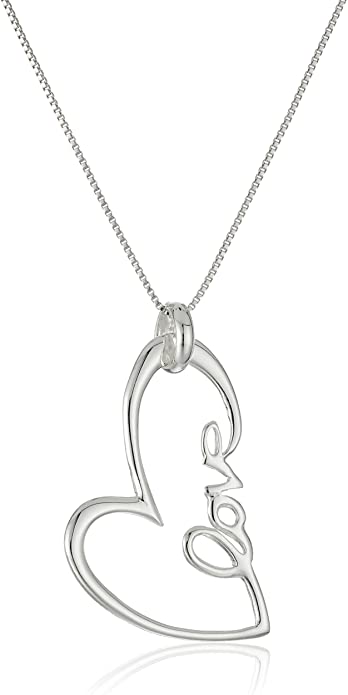
\includegraphics[width=1.3cm]{bilder/necklace.jpg} \textbf{Produkt:} Sterling Silver \glqq{}Love\grqq{} Open Heart Pendant Necklace, 18\grqq{} \\ \\
        \textbf{\textsc{BiMeanVAE} COOP+Attribute-Model:} \ccolorbox[BackgroundColor]{ \textcolor{HighlightColor}{\strut This necklace}} \ccolorbox[BackgroundColor]{ \textcolor{HighlightColor}{\strut is a}} \ccolorbox[BackgroundColor]{ \textcolor{HighlightColor}{\strut great quality}} \textcolor{HighlightColor}{and} \textcolor{HighlightColor}{so} \textcolor{HighlightColor}{far} \textcolor{HighlightColor}{it}\textcolor{HighlightColor}{'s} \textcolor{HighlightColor}{the} perfect \textcolor{HighlightColor}{size}\ccolorbox[BackgroundColor]{\textcolor{HighlightColor}{\strut . It}} \ccolorbox[BackgroundColor]{ \textcolor{HighlightColor}{\strut is a}} \textcolor{HighlightColor}{very} \textcolor{HighlightColor}{nice} \textcolor{HighlightColor}{looking} \textcolor{HighlightColor}{necklace}\textcolor{HighlightColor}{,} \ccolorbox[BackgroundColor]{ \textcolor{HighlightColor}{\strut and the}} color \underline{\ccolorbox[BackgroundColor]{ \textcolor{HighlightColor}{\strut is beautiful}}\ccolorbox[BackgroundColor]{ \textcolor{HighlightColor}{\strut. The}} \ccolorbox[BackgroundColor]{ \textcolor{HighlightColor}{\strut chain is}} \textcolor{HighlightColor}{a}} perfect gift \ccolorbox[BackgroundColor]{ \textcolor{HighlightColor}{\strut for the}} \textcolor{HighlightColor}{price} \textcolor{HighlightColor}{of} \textcolor{HighlightColor}{the} necklace. I love \textcolor{HighlightColor}{it}\textcolor{HighlightColor}{!} \\ 
        \textbf{Scores:} R-1: 48.63, R-2: 16.78, R-L: 28.08, MV: 60.05\\ \\
        %\textbf{\textsc{BiMeanVAE} COOP:} \textcolor{HighlightColor}{This} \ccolorbox[BackgroundColor]{ \textcolor{HighlightColor}{\strut is a}} \textcolor{HighlightColor}{great} product \underline{\ccolorbox[BackgroundColor]{ \textcolor{HighlightColor}{\strut for the}} \ccolorbox[BackgroundColor]{ \textcolor{HighlightColor}{\strut price .}}} \textcolor{HighlightColor}{It} \ccolorbox[BackgroundColor]{ \textcolor{HighlightColor}{\strut is a}} \textcolor{HighlightColor}{very} \textcolor{HighlightColor}{good} \textcolor{HighlightColor}{quality} \textcolor{HighlightColor}{,} \ccolorbox[BackgroundColor]{ \textcolor{HighlightColor}{\strut and the}} \textcolor{HighlightColor}{price} was right \ccolorbox[BackgroundColor]{ \textcolor{HighlightColor}{\strut . The}} only thing \textcolor{HighlightColor}{is} that \ccolorbox[BackgroundColor]{ \textcolor{HighlightColor}{\strut it is}} \textcolor{HighlightColor}{a} little small \ccolorbox[BackgroundColor]{ \textcolor{HighlightColor}{\strut , but}} \textcolor{HighlightColor}{it} \textcolor{HighlightColor}{'s} not too big \ccolorbox[BackgroundColor]{ \textcolor{HighlightColor}{\strut . It}} \textcolor{HighlightColor}{'s} \ccolorbox[BackgroundColor]{ \textcolor{HighlightColor}{\strut a great}} buy \ccolorbox[BackgroundColor]{ \textcolor{HighlightColor}{\strut for the}} \ccolorbox[BackgroundColor]{ \textcolor{HighlightColor}{\strut price .}}  \\ 
        %\textbf{Scores:} R-1: 36.61, R-2: 8.30, R-L: 26.44, MV: 55.57 \\ \\
        \textbf{\textsc{BiMeanVAE} COOP:} \textcolor{HighlightColor}{It} was \textcolor{HighlightColor}{a} perfect gift \ccolorbox[BackgroundColor]{ \textcolor{HighlightColor}{for a}} friend \textcolor{HighlightColor}{of} her birthday\textcolor{HighlightColor}{.} She loves \textcolor{HighlightColor}{it}\textcolor{HighlightColor}{,} \textcolor{HighlightColor}{the} \textcolor{HighlightColor}{look} \textcolor{HighlightColor}{is} \textcolor{HighlightColor}{great}\textcolor{HighlightColor}{,} \ccolorbox[BackgroundColor]{ \textcolor{HighlightColor}{and the}} \textcolor{HighlightColor}{price} was \textcolor{HighlightColor}{great}\ccolorbox[BackgroundColor]{\textcolor{HighlightColor}{. It}} was easy \textcolor{HighlightColor}{to} set up\textcolor{HighlightColor}{,} \textcolor{HighlightColor}{and} she loves it. I \underline{\ccolorbox[BackgroundColor]{ \textcolor{HighlightColor}{would recommend}} \textcolor{HighlightColor}{this}} product \ccolorbox[BackgroundColor]{ \textcolor{HighlightColor}{to anyone}}\textcolor{HighlightColor}{.}   \\ 
        \textbf{Scores:} R-1: 33.56, R-2: 5.71, R-L: 20.27, MV: 56.00 \\ \\
    

        \textbf{Optimus COOP+Attribute-Model:} \textcolor{HighlightColor}{This} \ccolorbox[BackgroundColor]{ \textcolor{HighlightColor}{\strut is a}} \textcolor{HighlightColor}{great} gift \underline{\ccolorbox[BackgroundColor]{ \textcolor{HighlightColor}{\strut for the}} \ccolorbox[BackgroundColor]{ \textcolor{HighlightColor}{\strut price.}}} She loves \textcolor{HighlightColor}{it}\textcolor{HighlightColor}{,} \textcolor{HighlightColor}{so} much better than \textcolor{HighlightColor}{the} \textcolor{HighlightColor}{necklace} \textcolor{HighlightColor}{and} \textcolor{HighlightColor}{it} looks \ccolorbox[BackgroundColor]{ \textcolor{HighlightColor}{\strut beautiful.}} You \textcolor{HighlightColor}{can't} \textcolor{HighlightColor}{get} \textcolor{HighlightColor}{a} gift on \ccolorbox[BackgroundColor]{ \textcolor{HighlightColor}{\strut the chain}} \ccolorbox[BackgroundColor]{ \textcolor{HighlightColor}{\strut, but}} \ccolorbox[BackgroundColor]{ \textcolor{HighlightColor}{\strut it is}} not worth \textcolor{HighlightColor}{the} money\textcolor{HighlightColor}{!} \textcolor{HighlightColor}{It} looks \textcolor{HighlightColor}{great}\textcolor{HighlightColor}{!}         \\ 
        \textbf{Scores:} R-1: 42.65, R-2: 9.28, R-L: 26.57, MV: 58.31\\ \\
        % \textbf{Optimus COOP:}  \ So \textcolor{HighlightColor}{far} \textcolor{HighlightColor}{the} \underline{\ccolorbox[BackgroundColor]{ \textcolor{HighlightColor}{\strut necklace is}} \textcolor{HighlightColor}{beautiful}} \textcolor{HighlightColor}{,} \ccolorbox[BackgroundColor]{ \textcolor{HighlightColor}{\strut and the}} perfect gift \textcolor{HighlightColor}{for} someone who \ccolorbox[BackgroundColor]{ \textcolor{HighlightColor}{\strut is a}} \ccolorbox[BackgroundColor]{ \textcolor{HighlightColor}{\strut beautiful piece}} \ccolorbox[BackgroundColor]{ \textcolor{HighlightColor}{\strut . It}} looks \textcolor{HighlightColor}{great} on \textcolor{HighlightColor}{the} picture \ccolorbox[BackgroundColor]{ \textcolor{HighlightColor}{\strut , but}} \textcolor{HighlightColor}{it} does not \textcolor{HighlightColor}{look} like \textcolor{HighlightColor}{a} gift \textcolor{HighlightColor}{.} Im \textcolor{HighlightColor}{very} happy with \textcolor{HighlightColor}{this} \textcolor{HighlightColor}{necklace} \textcolor{HighlightColor}{and} \ccolorbox[BackgroundColor]{ \textcolor{HighlightColor}{\strut it is}} not worth \textcolor{HighlightColor}{the} money \textcolor{HighlightColor}{!}  \\ 
        % \textbf{Scores:} R-1: 40.26, R-2: 13.01, R-L: 23.48, MV: 58.06 }
        \textbf{Optimus COOP:}  Its \ccolorbox[BackgroundColor]{ \textcolor{HighlightColor}{a beautiful}} \textcolor{HighlightColor}{necklace}\textcolor{HighlightColor}{,} \textcolor{HighlightColor}{and} \textcolor{HighlightColor}{it} looks \textcolor{HighlightColor}{great} \underline{\ccolorbox[BackgroundColor]{ \textcolor{HighlightColor}{for the}} \ccolorbox[BackgroundColor]{ \textcolor{HighlightColor}{price.}}} She said \textcolor{HighlightColor}{it} was \textcolor{HighlightColor}{a} gift \textcolor{HighlightColor}{for} her birthday present\ccolorbox[BackgroundColor]{\textcolor{HighlightColor}{, but}} \ccolorbox[BackgroundColor]{ \textcolor{HighlightColor}{it is}} \textcolor{HighlightColor}{very} \textcolor{HighlightColor}{thin} \textcolor{HighlightColor}{and} not worth \textcolor{HighlightColor}{the} money\textcolor{HighlightColor}{.} If \textcolor{HighlightColor}{you} want \textcolor{HighlightColor}{to} go wrong with \textcolor{HighlightColor}{this} \textcolor{HighlightColor}{necklace}\textcolor{HighlightColor}{!}  \\ 
        \textbf{Scores:} R-1: 37.76, R-2: 8.57, R-L: 21.67, MV: 57.69 }
    
        }
    \caption{Vergleich der generierten Rezensionen zwischen dem COOP und COOP + Attributionsmodell zu Produkt B0040EIHQQ des Amazon Datensatzes}
\label{reviewAmz1}
\end{Rezension}

Die in Rezension \ref{reviewAmz1} generierten Rezensionen für eine Halskette des Amazons Datensatzes zeigen insgesamt gute Ergebnisse.
Der Inhalt der beiden durch \textsc{BiMeanVAE} generierten Rezensionen ist konsistent. 
Das Sentiment ist positiv und die Kette wird abschließend zum Kaufen empfohlen. Besonders auffällig ist die höhere Präzision des Attributmodells. Das Produkt und die Eigenschaften dieses werden explizit erwähnt, wie zum Beispiel durch \glqq{}great quality\grqq{}, \glqq{}perfect size\grqq{}, \glqq{}very nice looking necklace\grqq{}, \glqq{}color is beautiful\grqq{} und \glqq{}perfect gift for the price\grqq{}.
Im Gegensatz dazu ist die vom COOP Modell generierte Rezension allgemeiner und erwähnt lediglich das gute Aussehen der Halskette \glqq{}the look is great\grqq{} und den Preis \glqq{}price was great\grqq{} des Produktes ohne auf spezifische Eigenschaften des Produktes wie zum Beispiel die Farbe einzugehen.
Diese Auswertung spiegelt sich auch in den Metriken wieder, in denen das Attributmodell die Metriken des COOP Modells in allen Werten übertrifft. 
Insbesondere der Moverscore, der die semantische Ähnlichkeit zu den Gold-Zusammenfassungen angibt, ist mit 60.05 beim Attributmodell bedeutend höher als die 56.00 des COOP Modells.
In dieser Beispielrezension bestätigt sich die Hypothese, dass das Attributmodell durch geeignete Tokens in einem Bag of Words Modell die Generierung präzise konditionieren können.

Die durch Optimus erstellten Rezensionen sind sowohl beim COOP, wie auch beim Attributmodell inkonsistent in ihrem Inhalt. 
Die Rezensionen haben beide hauptsächlich ein positives Sentiment, widersprechen sich allerdings beide jeweils mit den Formulierungen \glqq{}great for the price\grqq{} und \glqq{}not worth the money\grqq{}.
Trotzdem gehen beide Modelle auf unterschiedliche Aspekte der zu bewertenden Halskette ein und beschreiben den Stil der Kette als \glqq{}it looks beautiful\grqq{}, \glqq{}It looks great!\grqq{} und \glqq{}a beautiful necklace\grqq{}.
Eine Steigerung der Leistung der generierten Rezensionen des Attributmodells gegenüber dem COOP Modell kann hier nur an den Metriken festgestellt werden und spiegelt sich nur minimal in der generierten Rezension wieder.
Hier fällt auf, dass das Attributmodell versucht die Kette \glqq{}the chain\grqq{} der Halskette anzusprechen, allerdings keinen semantisch korrekten Satz mit diesen Tokens bildet.

\begin{Rezension}[!h]
    \centering
    %\scriptsize
    \small
    \framebox{
        \parbox{\columnwidth-4\fboxsep}{
            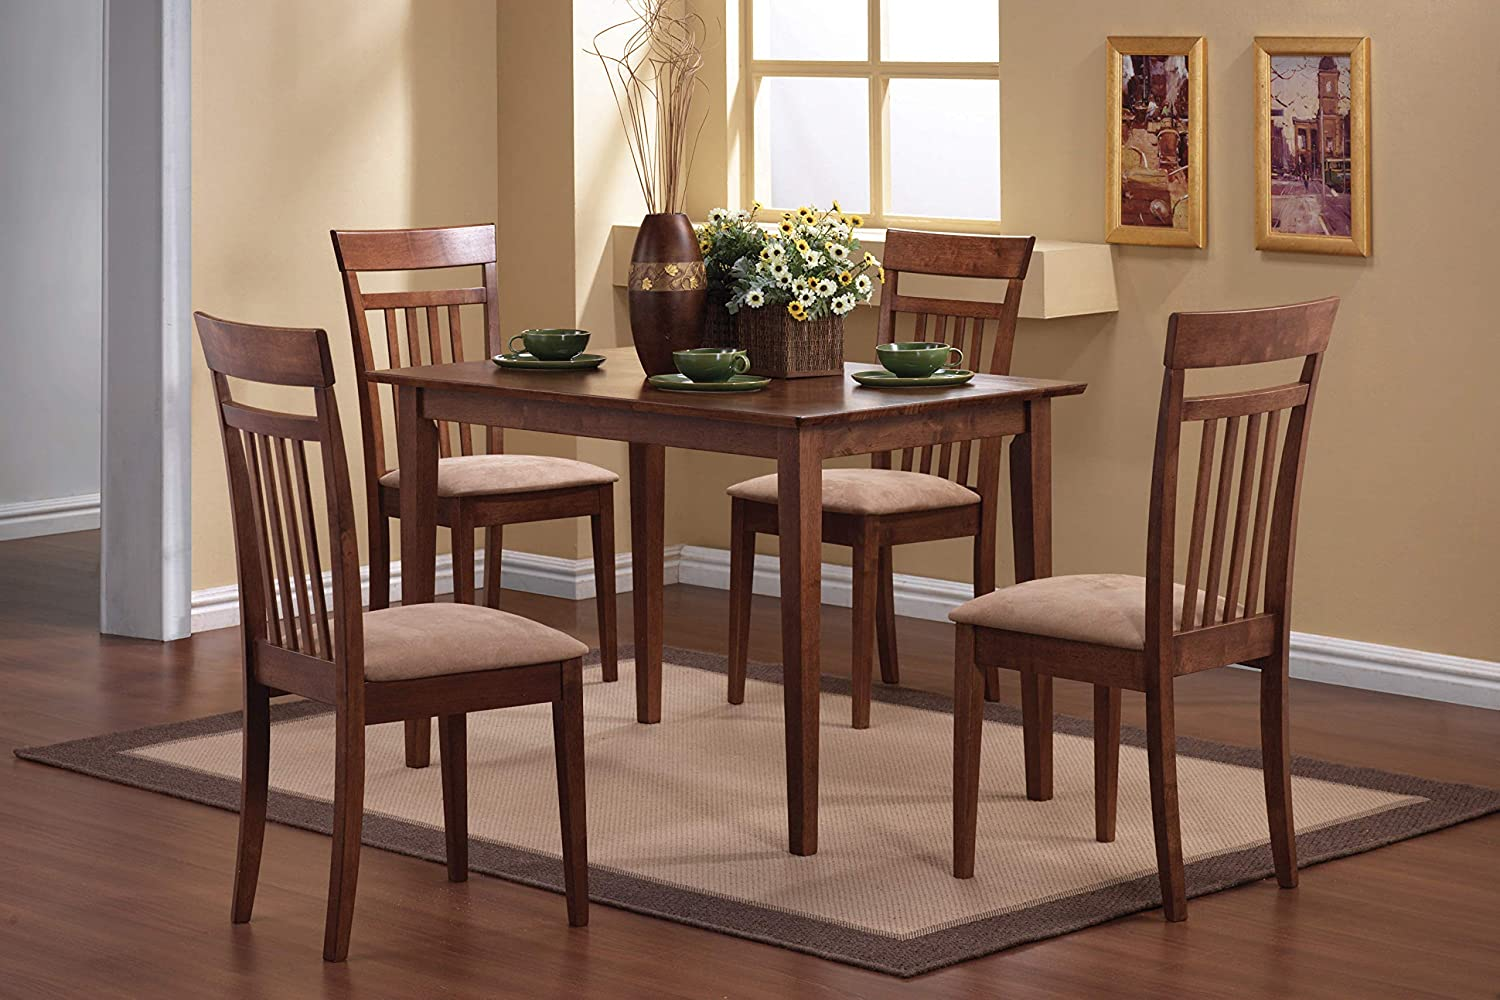
\includegraphics[width=1.5cm]{bilder/table.jpg} \textbf{Produkt:} Coaster CO-150430 5 Pc Dining Set, Chestnut \\ \\
        \textbf{\textsc{BiMeanVAE} COOP+Attribute-Model:} \textcolor{HighlightColor}{The} table \ccolorbox[BackgroundColor]{ \textcolor{HighlightColor}{is very}} \textcolor{HighlightColor}{nice} \textcolor{HighlightColor}{and} \textcolor{HighlightColor}{sturdy}\ccolorbox[BackgroundColor]{\textcolor{HighlightColor}{. It}} \textcolor{HighlightColor}{was} \ccolorbox[BackgroundColor]{ \textcolor{HighlightColor}{easy to}} \ccolorbox[BackgroundColor]{ \textcolor{HighlightColor}{put together}} \textcolor{HighlightColor}{and} \textcolor{HighlightColor}{the} \textcolor{HighlightColor}{color} \textcolor{HighlightColor}{is} perfect\ccolorbox[BackgroundColor]{\textcolor{HighlightColor}{. The}} \textcolor{HighlightColor}{chairs} \textcolor{HighlightColor}{are} \textcolor{HighlightColor}{a} bit \textcolor{HighlightColor}{small} \textcolor{HighlightColor}{for} \textcolor{HighlightColor}{the} price\ccolorbox[BackgroundColor]{\textcolor{HighlightColor}{, but}} \textcolor{HighlightColor}{it}'s \textcolor{HighlightColor}{not} \textcolor{HighlightColor}{a} big \textcolor{HighlightColor}{deal}\ccolorbox[BackgroundColor]{\textcolor{HighlightColor}{. It}} \textcolor{HighlightColor}{was} \underline{\ccolorbox[BackgroundColor]{ \textcolor{HighlightColor}{very easy}} \ccolorbox[BackgroundColor]{ \textcolor{HighlightColor}{to assemble}}\textcolor{HighlightColor}{.}}        \\ 
        \textbf{Scores:} R-1: 42.75, R-2: 7.03, R-L: 23.66, MV: 54.49\\ \\
        \textbf{\textsc{BiMeanVAE} COOP:} \textcolor{HighlightColor}{The} table \ccolorbox[BackgroundColor]{ \textcolor{HighlightColor}{is very}} \textcolor{HighlightColor}{nice} \textcolor{HighlightColor}{and} \textcolor{HighlightColor}{sturdy}\ccolorbox[BackgroundColor]{\textcolor{HighlightColor}{. The}} \textcolor{HighlightColor}{chairs} \textcolor{HighlightColor}{are} \underline{\ccolorbox[BackgroundColor]{ \textcolor{HighlightColor}{easy to}} \ccolorbox[BackgroundColor]{ \textcolor{HighlightColor}{put together}}} \textcolor{HighlightColor}{and} \textcolor{HighlightColor}{the} \textcolor{HighlightColor}{color} \textcolor{HighlightColor}{is} \textcolor{HighlightColor}{great}\ccolorbox[BackgroundColor]{\textcolor{HighlightColor}{. It}} \textcolor{HighlightColor}{was} \ccolorbox[BackgroundColor]{ \textcolor{HighlightColor}{easy to}} \textcolor{HighlightColor}{assemble}\textcolor{HighlightColor}{,} \textcolor{HighlightColor}{and} \textcolor{HighlightColor}{the} price \textcolor{HighlightColor}{was} right\ccolorbox[BackgroundColor]{\textcolor{HighlightColor}{. The}} \textcolor{HighlightColor}{size} \textcolor{HighlightColor}{is} perfect \ccolorbox[BackgroundColor]{ \textcolor{HighlightColor}{for a}} \textcolor{HighlightColor}{small} kitchen\textcolor{HighlightColor}{,} \textcolor{HighlightColor}{so} \textcolor{HighlightColor}{it}'s \textcolor{HighlightColor}{not} \textcolor{HighlightColor}{a} big \textcolor{HighlightColor}{deal}\textcolor{HighlightColor}{.}         \\ 
        \textbf{Scores:} R-1: 41.60, R-2: 9.70, R-L: 24.81, MV: 54.53 \\ \\

        \textbf{Optimus COOP+Attribute-Model:} Just received this table \textcolor{HighlightColor}{top} \textcolor{HighlightColor}{and} \textcolor{HighlightColor}{sturdy}\ccolorbox[BackgroundColor]{\textcolor{HighlightColor}{. The}} table \textcolor{HighlightColor}{is} perfect \textcolor{HighlightColor}{for} \textcolor{HighlightColor}{the} price\textcolor{HighlightColor}{,} \textcolor{HighlightColor}{so} \textcolor{HighlightColor}{it} \textcolor{HighlightColor}{was} \underline{\ccolorbox[BackgroundColor]{ \textcolor{HighlightColor}{easy to}}\ccolorbox[BackgroundColor]{\textcolor{HighlightColor}{assemble.}}} One \ccolorbox[BackgroundColor]{ \textcolor{HighlightColor}{of the}} \textcolor{HighlightColor}{chairs} \textcolor{HighlightColor}{are} \textcolor{HighlightColor}{not} \ccolorbox[BackgroundColor]{ \textcolor{HighlightColor}{sturdy,}} \textcolor{HighlightColor}{sturdy} \textcolor{HighlightColor}{and} \textcolor{HighlightColor}{the} table \textcolor{HighlightColor}{was} \textcolor{HighlightColor}{not} worth \textcolor{HighlightColor}{the} money\textcolor{HighlightColor}{.} Other than \ccolorbox[BackgroundColor]{ \textcolor{HighlightColor}{that it}} \textcolor{HighlightColor}{is} \textcolor{HighlightColor}{a} \textcolor{HighlightColor}{great} \ccolorbox[BackgroundColor]{ \textcolor{HighlightColor}{purchase.}}         \\ 
        \textbf{Scores:} R-1: 32.85, R-2: 5.22, R-L: 20.44, MV: 53.52 \\ \\
        \textbf{Optimus COOP:} Just received this table \textcolor{HighlightColor}{and} \textcolor{HighlightColor}{sturdy}\ccolorbox[BackgroundColor]{\textcolor{HighlightColor}{. The}} table \textcolor{HighlightColor}{is} perfect \textcolor{HighlightColor}{for} \textcolor{HighlightColor}{the} price\textcolor{HighlightColor}{,} \ccolorbox[BackgroundColor]{ \textcolor{HighlightColor}{and it}} \textcolor{HighlightColor}{was} \underline{\ccolorbox[BackgroundColor]{ \textcolor{HighlightColor}{easy to}} \ccolorbox[BackgroundColor]{ \textcolor{HighlightColor}{assemble.}}} One \ccolorbox[BackgroundColor]{ \textcolor{HighlightColor}{of the}} \textcolor{HighlightColor}{chairs} \textcolor{HighlightColor}{are} \textcolor{HighlightColor}{not} perfect\ccolorbox[BackgroundColor]{\textcolor{HighlightColor}{. It}} \textcolor{HighlightColor}{is} \textcolor{HighlightColor}{sturdy} \textcolor{HighlightColor}{and} \textcolor{HighlightColor}{not} worth \textcolor{HighlightColor}{the} money\textcolor{HighlightColor}{.}         \\ 
        \textbf{Scores:} R-1: 30.32, R-2: 6.72, R-L: 19.67, MV: 53.49 }
    }
    \caption{Vergleich der generierten Rezensionen zwischen dem COOP und COOP+Attributmodell zu Produkt B001EQJ5AU des Amazon Datensatzes}
    \label{reviewAmz2}
\end{Rezension}

Rezension \ref{reviewAmz2} bewertet ein Set bestehend aus einem Tisch und 4 Stühlen.
Die durch \textsc{BiMeanVAE} generierten Rezensionen sind in ihrem Inhalt konsistent und beschreiben präzise den Inhalt des Sets.
Beide Rezensionen erwähnen die Eigenschaften \glqq{}easy to put together\grqq{}, \glqq{}easy to assemble\grqq{}, die Farbe und die Qualität des Sets.
Somit werden die einzelnen Aspekte des Produktes in den beiden Rezensionen aufgegriffen.
Anschaulich ist die Optimierung des Attributmodells der Phrase \glqq{}it's not a big deal\grqq{} semantisch korrekt zu Integrieren und den Bezug zur Größe der Stühle zu setzen.
Das COOP Modell widerspricht sich hier in der Semantik mit \glqq{}The size is perfect for a small kitchen, so it's not a big deal\grqq{}, da kein negativer Punkt angesprochen wird.
In den Metriken erzielen beide Modelle gute Ergebnisse, wobei das Attributmodell einen höheren ROUGE-1 Score hat und das COOP Modell in den anderen Metriken bessere Ergebnisse erzielt.

Die durch Optimus erzeugten Rezensionen beschreiben ebenfalls den Inhalt des Sets und erwähnen die Eigenschaften \glqq{}easy to assemble\grqq{} und die Qualität.
Teilweise sind die erzeugten Sätze syntaktisch nicht korrekt. 
In diesem Beispiel ist erkennbar, dass das Attributmodell höchstwahrscheinlich ab der Stelle \glqq{}One of the chairs\grqq{} die Tokens bei der Generierung stark beeinflusst hat und somit die Semantik des verbleibenden Teils positiv beeinflusst hat.
In den Metriken erzielt das Attributmodell in allen Metriken, außer dem ROUGE-2 Score, bessere Ergebnisse.

% \begin{Rezension}[!h]
%     \centering
%     %\scriptsize
%     \small
%     \framebox{
%         \parbox{\columnwidth-4\fboxsep}{
%             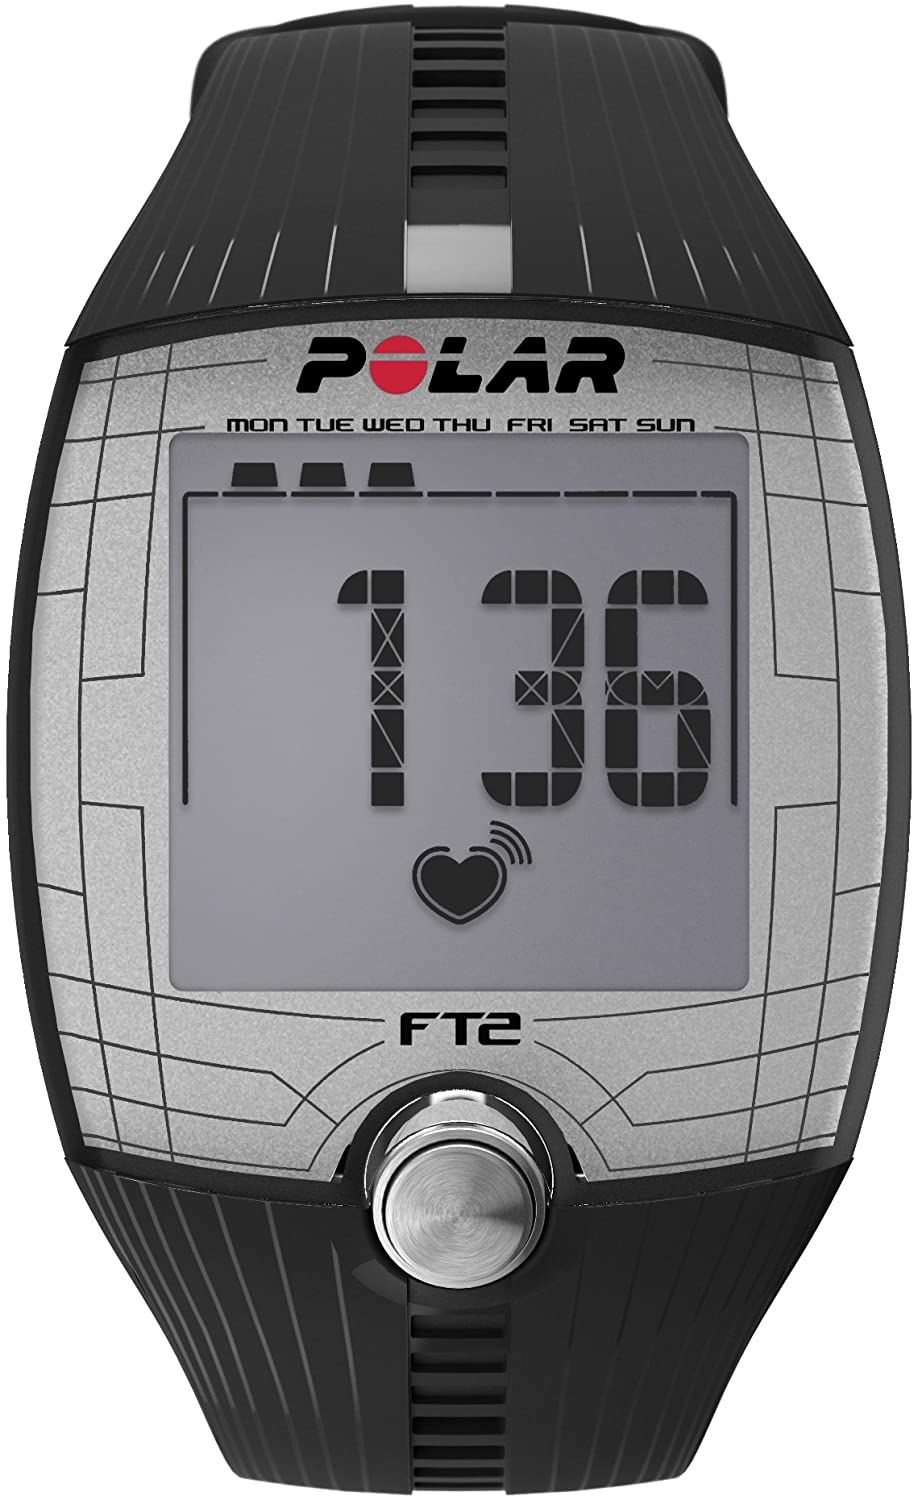
\includegraphics[width=1.5cm]{bilder/polarfit.jpg} \textbf{Produkt:} Polar FT2 Heart Rate Monitor \\ \\
%         \textbf{\textsc{BiMeanVAE} COOP+Attribute-Model:} If \ccolorbox[BackgroundColor]{ \textcolor{HighlightColor}{\strut you are}} looking \textcolor{HighlightColor}{for} \underline{\ccolorbox[BackgroundColor]{ \textcolor{HighlightColor}{\strut a heart}} \ccolorbox[BackgroundColor]{ \textcolor{HighlightColor}{\strut rate monitor}}} \textcolor{HighlightColor}{this} \ccolorbox[BackgroundColor]{ \textcolor{HighlightColor}{\strut is the}} best \ccolorbox[BackgroundColor]{ \textcolor{HighlightColor}{\strut . It}} 's \ccolorbox[BackgroundColor]{ \textcolor{HighlightColor}{\strut easy to}} \textcolor{HighlightColor}{use} \textcolor{HighlightColor}{,} \textcolor{HighlightColor}{and} \textcolor{HighlightColor}{it} works great \ccolorbox[BackgroundColor]{ \textcolor{HighlightColor}{\strut . The}} \textcolor{HighlightColor}{only} downside \textcolor{HighlightColor}{is} \textcolor{HighlightColor}{that} \textcolor{HighlightColor}{you} have \textcolor{HighlightColor}{to} \textcolor{HighlightColor}{be} careful \textcolor{HighlightColor}{not} \textcolor{HighlightColor}{to} take \textcolor{HighlightColor}{it} \ccolorbox[BackgroundColor]{ \textcolor{HighlightColor}{\strut out of}} \textcolor{HighlightColor}{the} \textcolor{HighlightColor}{case} \textcolor{HighlightColor}{.} \\ 
%         \textbf{Scores:} R-1: 39.26, R-2: 13.12, R-L: 22.08, MV: 56.40\\ \\
%         \textbf{\textsc{BiMeanVAE} COOP:} \ccolorbox[BackgroundColor]{ \textcolor{HighlightColor}{\strut This is}} \textcolor{HighlightColor}{a} great \textcolor{HighlightColor}{product} \ccolorbox[BackgroundColor]{ \textcolor{HighlightColor}{\strut . It}} was \ccolorbox[BackgroundColor]{ \textcolor{HighlightColor}{\strut easy to}} \ccolorbox[BackgroundColor]{ \textcolor{HighlightColor}{\strut set up}} \textcolor{HighlightColor}{and} \ccolorbox[BackgroundColor]{ \textcolor{HighlightColor}{\strut use .}} \ccolorbox[BackgroundColor]{ \textcolor{HighlightColor}{\strut The only}} downside \textcolor{HighlightColor}{is} \textcolor{HighlightColor}{that} \textcolor{HighlightColor}{it} 's \textcolor{HighlightColor}{a} little hard \textcolor{HighlightColor}{to} get \textcolor{HighlightColor}{on} \textcolor{HighlightColor}{and} off \ccolorbox[BackgroundColor]{ \textcolor{HighlightColor}{\strut , but}} \textcolor{HighlightColor}{it} 's \textcolor{HighlightColor}{not} \textcolor{HighlightColor}{a} problem \ccolorbox[BackgroundColor]{ \textcolor{HighlightColor}{\strut . It}} \underline{\ccolorbox[BackgroundColor]{ \textcolor{HighlightColor}{\strut is easy}} \ccolorbox[BackgroundColor]{ \textcolor{HighlightColor}{\strut to use}}} \textcolor{HighlightColor}{and} \textcolor{HighlightColor}{the} price \textcolor{HighlightColor}{is} right \textcolor{HighlightColor}{.}         \\ 
%         \textbf{Scores:} R-1: 28.99, R-2: 7.83, R-L: 20.11, MV: 54.33 \\ \\

%         \textbf{Optimus COOP+Attribute-Model:} \underline{\ccolorbox[BackgroundColor]{ \textcolor{HighlightColor}{\strut This is}} \ccolorbox[BackgroundColor]{ \textcolor{HighlightColor}{\strut a good}}} price \ccolorbox[BackgroundColor]{ \textcolor{HighlightColor}{\strut . You}} ca \textcolor{HighlightColor}{n't} \textcolor{HighlightColor}{be} able \ccolorbox[BackgroundColor]{ \textcolor{HighlightColor}{\strut to use}} \textcolor{HighlightColor}{it} \textcolor{HighlightColor}{in} \textcolor{HighlightColor}{your} \ccolorbox[BackgroundColor]{ \textcolor{HighlightColor}{\strut heart rate}} \ccolorbox[BackgroundColor]{ \textcolor{HighlightColor}{\strut monitor ,}} \textcolor{HighlightColor}{which} \ccolorbox[BackgroundColor]{ \textcolor{HighlightColor}{\strut is very}} \textcolor{HighlightColor}{accurate} \textcolor{HighlightColor}{.} If \ccolorbox[BackgroundColor]{ \textcolor{HighlightColor}{\strut you need}} \textcolor{HighlightColor}{to} \textcolor{HighlightColor}{be} aware \textcolor{HighlightColor}{that} \textcolor{HighlightColor}{you} have \ccolorbox[BackgroundColor]{ \textcolor{HighlightColor}{\strut to read}} all \textcolor{HighlightColor}{the} reviews \textcolor{HighlightColor}{and} \textcolor{HighlightColor}{it} 's \textcolor{HighlightColor}{very} comfortable \ccolorbox[BackgroundColor]{ \textcolor{HighlightColor}{\strut . It}} \ccolorbox[BackgroundColor]{ \textcolor{HighlightColor}{\strut is easy}} \textcolor{HighlightColor}{to} \ccolorbox[BackgroundColor]{ \textcolor{HighlightColor}{\strut set up}} \textcolor{HighlightColor}{and} \textcolor{HighlightColor}{you} \textcolor{HighlightColor}{can} \textcolor{HighlightColor}{use} \textcolor{HighlightColor}{the} \ccolorbox[BackgroundColor]{ \textcolor{HighlightColor}{\strut monitor .}} \\ 
%         \textbf{Scores:} R-1: 42.73, R-2: 12.25, R-L: 24.65, MV: 57.76 \\ \\
%         \textbf{Optimus COOP:} \textcolor{HighlightColor}{It} 's \ccolorbox[BackgroundColor]{ \textcolor{HighlightColor}{\strut very} \underline{\textcolor{HighlightColor}{easy}}}\underline{ \ccolorbox[BackgroundColor]{ \textcolor{HighlightColor}{\strut to use}}} \textcolor{HighlightColor}{.} After reading \textcolor{HighlightColor}{the} reviews \textcolor{HighlightColor}{and} \ccolorbox[BackgroundColor]{ \textcolor{HighlightColor}{\strut it is}} \textcolor{HighlightColor}{very} \textcolor{HighlightColor}{accurate} \textcolor{HighlightColor}{.} If \textcolor{HighlightColor}{you} 're looking \textcolor{HighlightColor}{for} \textcolor{HighlightColor}{a} regular basis \textcolor{HighlightColor}{,} \textcolor{HighlightColor}{you} \textcolor{HighlightColor}{can} see \ccolorbox[BackgroundColor]{ \textcolor{HighlightColor}{\strut if you}} \textcolor{HighlightColor}{need} \textcolor{HighlightColor}{to} change \textcolor{HighlightColor}{the} \ccolorbox[BackgroundColor]{ \textcolor{HighlightColor}{\strut monitor .}} \textcolor{HighlightColor}{The} \ccolorbox[BackgroundColor]{ \textcolor{HighlightColor}{\strut monitor is}} \textcolor{HighlightColor}{that} \textcolor{HighlightColor}{it} 's \textcolor{HighlightColor}{not} too bulky \ccolorbox[BackgroundColor]{ \textcolor{HighlightColor}{\strut . Very}} happy \textcolor{HighlightColor}{with} \ccolorbox[BackgroundColor]{ \textcolor{HighlightColor}{\strut this product}} \textcolor{HighlightColor}{and} \textcolor{HighlightColor}{will} \textcolor{HighlightColor}{be} reccomend \textcolor{HighlightColor}{it} \textcolor{HighlightColor}{.}  \\ 
%         \textbf{Scores:} R-1: 38.67, R-2: 8.98, R-L: 22.09, MV: 57.13 }
    
%     }
%     \caption{Vergleich der generierten Rezensionen zwischen dem COOP und COOP+Attributmodell zu Produkt B003HT9W32 des Amazon Datensatzes}
%     \label{reviewAmz2}
% \end{Rezension}


% Rezension \ref{reviewAmz2} bewertet eine Fitness Puls Uhr des Amazon Datensatzes.
% Die durch \textsc{BiMeanVAE} generierten Rezensionen sind in ihrem Inhalt konsistent und haben ein positives Sentiment. 
% Beide Rezensionen erwähnen ähnliche Eigenschaften der Bedienungsfreundlichkeit \glqq{}easy to use\grqq{}, \glqq{}easy to setup and use\grqq{} und der Funktionalität \glqq{}it works great\grqq{}, \glqq{}great product\grqq{}.
% Ebenfalls erwähnen beide generierten Rezensionen jeweils einen validen negativen Punkt der Fitness Uhr.
% Somit gehen die Rezensionen präzise auf die Aspekte der Fitness Uhr ein. 
% Die durch das Attributmodell generierte Rezension erwähnt, dass es sich um einen \glqq{}heart rate monitor\grqq{} handelt, wodurch diese Rezension noch präziser ist.
% Dies ist auch in den Metriken zu erkennen, in denen das Attributmodell in allen Metriken eine bessere Leistung als das COOP Modell erzielt.

% Die durch Optimus erzeugten Rezensionen haben eine schlechtere Konsistenz im Inhalt. 
% Hier existieren sinnvolle Teilbereiche die auf Eigenschaften eingehen wie zum Beispiel \glqq{}is very accurate\grqq{}, allerdings wiedersprechen sich in beiden Rezensionen einige Fakten und bauen nicht konsistent aufeinander auf.
% Beide Rezensionen erwähnen, dass es sich bei dem Produkt um einen \glqq{}heart rate monitor\grqq{} handelt.
% Trotz der manuell evaluierten schlechteren Konsistenz des Inhaltes weisen beide Rezensionen bessere Metriken auf als die \textsc{BiMeanVAE} Modelle, wobei auch hier bei den Optimus Modellen das Attributmodell die besten Metriken erzielt. 
% Wie auch bei Rezension \ref{reviewAmz1} zeigt hier das Attributmodell bei Optimus lediglich eine äußerst geringe Leistungssteigerung in der manuellen Evaluation, da zwar durch das Attributmodell spezielle Wörter wie \glqq{}heart rate monitor\grqq{} im Gegensatz zu \glqq{}monitor\grqq{} forciert werden, die Rezensionen trotzdem aber noch inkonsistent im Inhalt sind.

Insgesamt zeigt auf dem Amazon Datensatz \textsc{BiMeanVAE} mit Attributmodell auf beiden Rezensionen \ref{reviewAmz1} und \ref{reviewAmz2} die besten Ergebnisse in Bezug auf konsistenten Inhalt, Semantik und präzisen Formulierungen der wichtigen Aspekte der Produkte.
Durch das Attributmodell sind die \textsc{BiMeanVAE} Rezensionen wesentlich ausdrucksstärker, da seltene Wörter, die in Bezug auf die Rezensionen eine hohe Relevanz haben, häufiger miteinbezogen werden.

\pagebreak
\subsubsection{Yelp Rezensionen} %idx 85, 67, 60 (great)
Nachfolgend werden zwei generierte Rezensionen des Yelp Datensatzes evaluiert. 
Bei dem Yelp Datensatz ist zu beachten, dass je Dienstleistung jeweils nur eine Referenzzusammenfassung existiert.
Demnach ist eine Vergleichbarkeit an Metriken nur unzureichend möglich, da insbesondere bei Textsequenzen Rouge Metriken die Semantik der Textsequenzen nicht erfassen.

\begin{Rezension}[!h] %60
    \centering
    %\scriptsize
    \small
    \framebox{
        \parbox{\columnwidth-4\fboxsep}{
        \textbf{Restaurant:} Harbour 60 Steakhouse \\ \\
        \textbf{Referenz:} This place has some amazing, tasty steaks!  They are breathtaking!  The menu also has seafood options that are just as delicious!  The only downside is that its pretty expensive, however you get top quality meat for what you pay for.  You won't even notice the price when your stomach is filled with the best seasoned meat you've ever had.
        \\ \\
        \textbf{\textsc{BiMeanVAE} COOP+Attribute-Model:} \underline{\ccolorbox[BackgroundColor]{ \textcolor{HighlightColor}{This place}}} \textcolor{HighlightColor}{is} a great \textcolor{HighlightColor}{place} to eat\textcolor{HighlightColor}{.} \textcolor{HighlightColor}{The} food \textcolor{HighlightColor}{is} very good and \textcolor{HighlightColor}{the} service \textcolor{HighlightColor}{is} excellent\textcolor{HighlightColor}{.} It's a little pricey but it's worth it \textcolor{HighlightColor}{for} \textcolor{HighlightColor}{the} \textcolor{HighlightColor}{quality} of \textcolor{HighlightColor}{the} food and \textcolor{HighlightColor}{the} service\textcolor{HighlightColor}{.} \textcolor{HighlightColor}{The} steak was cooked to perfection and \textcolor{HighlightColor}{the} lobster bisque was \textcolor{HighlightColor}{delicious}\textcolor{HighlightColor}{.} \textcolor{HighlightColor}{The} \textcolor{HighlightColor}{best} part of \textcolor{HighlightColor}{the} meal was \textcolor{HighlightColor}{the} wine\textcolor{HighlightColor}{.}         \\ 
        \textbf{Scores:} R-1: 21.85, R-2: 5.13, R-L: 15.13, MV: 56.57\\ \\
        \textbf{\textsc{BiMeanVAE} COOP:} Excellent food and great service\textcolor{HighlightColor}{.} \textcolor{HighlightColor}{The} staff \textcolor{HighlightColor}{is} very friendly and \textcolor{HighlightColor}{the} food \textcolor{HighlightColor}{is} \textcolor{HighlightColor}{delicious}\textcolor{HighlightColor}{.} \textcolor{HighlightColor}{The} steak was cooked to perfection and \textcolor{HighlightColor}{the} service was a little slow but it was worth \textcolor{HighlightColor}{the} wait\textcolor{HighlightColor}{.} It's a great \underline{\textcolor{HighlightColor}{place}} to go \textcolor{HighlightColor}{for} a date night\textcolor{HighlightColor}{.}         \\ 
        \textbf{Scores:} R-1: 18.86, R-2: 1.92, R-L: 9.43, MV: 55.69 \\ \\

        \textbf{Optimus COOP+Attribute-Model:} One of \underline{\ccolorbox[BackgroundColor]{ \textcolor{HighlightColor}{the best}}} steakhouse\textcolor{HighlightColor}{.} It's a great meal\textcolor{HighlightColor}{.} \textcolor{HighlightColor}{The} service was \textcolor{HighlightColor}{amazing} and \textcolor{HighlightColor}{the} food was \textcolor{HighlightColor}{delicious}\textcolor{HighlightColor}{.} If \textcolor{HighlightColor}{you}'re looking \textcolor{HighlightColor}{for} a long time to eat at \textcolor{HighlightColor}{the} strip\ccolorbox[BackgroundColor]{\textcolor{HighlightColor}{. You}} ca\textcolor{HighlightColor}{n't} wait \textcolor{HighlightColor}{for} dinner\textcolor{HighlightColor}{.} \textcolor{HighlightColor}{This} \textcolor{HighlightColor}{is} a little pricey \textcolor{HighlightColor}{for} \textcolor{HighlightColor}{the} steak and it was perfect\textcolor{HighlightColor}{.} Highly recommend this \textcolor{HighlightColor}{place} to anyone in town\textcolor{HighlightColor}{.}         \\ 
        \textbf{Scores:} R-1: 26.89, R-2: 3.42, R-L: 15.13, MV: 57.28 \\ \\
        \textbf{Optimus COOP:} \textcolor{HighlightColor}{This} restaurant \textcolor{HighlightColor}{is} a great \textcolor{HighlightColor}{place} to die \ccolorbox[BackgroundColor]{ \textcolor{HighlightColor}{for.}} \textcolor{HighlightColor}{The} food \textcolor{HighlightColor}{is} \textcolor{HighlightColor}{amazing} and \textcolor{HighlightColor}{the} service \textcolor{HighlightColor}{is} fantastic\textcolor{HighlightColor}{.} It's a little pricey but \textcolor{HighlightColor}{the} food was \textcolor{HighlightColor}{delicious}\textcolor{HighlightColor}{.} Everything was perfect \textcolor{HighlightColor}{for} \textcolor{HighlightColor}{the} steak and \underline{\ccolorbox[BackgroundColor]{ \textcolor{HighlightColor}{delicious!}} \textcolor{HighlightColor}{The}} service was great\textcolor{HighlightColor}{,} \ccolorbox[BackgroundColor]{ \textcolor{HighlightColor}{the best}} part of \textcolor{HighlightColor}{the} restaurant in \textcolor{HighlightColor}{the} city\textcolor{HighlightColor}{.} If \textcolor{HighlightColor}{you} want to go back \textcolor{HighlightColor}{for} dinner\textcolor{HighlightColor}{,} it's not worth it\textcolor{HighlightColor}{.}         \\ 
        \textbf{Scores:} R-1: 24.39, R-2: 3.30, R-L: 16.26, MV: 57.52  

        }
    }
    \caption{Vergleich der generierten Rezensionen zwischen dem COOP und COOP+Attributmodell zu Dienstleistung 4POPYEONJpkfhWOMx\_PyGg des Yelp Datensatzes} %4POPYEONJpkfhWOMx_PyGg
    \label{reviewYelp1}
\end{Rezension}

Rezension \ref{reviewYelp1} bewertet ein Steakhouse in Toronto. 
Insgesamt generieren alle Modelle gute Rezensionen und geben den Inhalt der Referenzbewertung wieder. 
Bei den durch \textsc{BiMeanVAE} generierten Bewertungen ist der Inhalt konsistent, das Essen und der Service wird als exzellent bewertet.
Die durch das Attributmodell erzeugte Rezension ist detaillierter und erwähnt zusätzlich noch den Wein und Hummer, der auch in der Referenz vorhanden ist. Ebenfalls erwähnt das Attributmodell die hohen Kosten, die auch in der Referenz vorkommen.
Die höhere Deckungsgleichheit ist auch in den Metriken wiederzufinden, in denen das Attributmodell in allen Metriken dem COOP Modell überlegen ist. 

Die Rezensionen der Optimus Modelle sind inhaltlich korrekt und erwähnen beide, dass es sich um ein delikates Steakhouse mit gutem Service handelt.
Das COOP Modell erzeugt in dieser Rezension teilweise untypische Formulierungen wie: \glqq{}This restaurant is a great place to die for\grqq{}.
In den Metriken sind die erzeugten Rezensionen der beiden Modelle ähnlich.

\begin{Rezension}[!h] %85
    \centering
    %\scriptsize
    \small
    \framebox{
        \parbox{\columnwidth-4\fboxsep}{
        \textbf{Restaurant:} Anna Marie's Italian Cuisine \\ \\
        \textbf{Referenz:} Great place to go food authentic Italian food. Pizza is amazing, lots of topping choices  and they aren't stingy with them. Drinks and desert wont disappoint either. The atmosphere is pleasant, and provides a nice escape from the heat. Staff can be hit or miss but the place is clean and they have some good happy hour deals.
        \\ \\
        \textbf{\textsc{BiMeanVAE} COOP+Attribute-Model:} Had \textcolor{HighlightColor}{a} great experience here\ccolorbox[BackgroundColor]{\textcolor{HighlightColor}{. The}} \textcolor{HighlightColor}{food} was very \textcolor{HighlightColor}{good} \textcolor{HighlightColor}{and} \textcolor{HighlightColor}{the} service was excellent\textcolor{HighlightColor}{.} It's \ccolorbox[BackgroundColor]{ \textcolor{HighlightColor}{a nice}} \underline{\ccolorbox[BackgroundColor]{ \textcolor{HighlightColor}{place to}} \textcolor{HighlightColor}{go}} \textcolor{HighlightColor}{with} \textcolor{HighlightColor}{a} group \textcolor{HighlightColor}{of} friends \textcolor{HighlightColor}{and} family\textcolor{HighlightColor}{.} They \textcolor{HighlightColor}{have} \textcolor{HighlightColor}{a} great \ccolorbox[BackgroundColor]{ \textcolor{HighlightColor}{happy hour}} menu \textcolor{HighlightColor}{and} \textcolor{HighlightColor}{the} \textcolor{HighlightColor}{food} \textcolor{HighlightColor}{is} very \textcolor{HighlightColor}{good}\textcolor{HighlightColor}{.} If you \textcolor{HighlightColor}{are} in \textcolor{HighlightColor}{the} area\textcolor{HighlightColor}{,} this \textcolor{HighlightColor}{is} \textcolor{HighlightColor}{a} must try\textcolor{HighlightColor}{.}         \\ 
        \textbf{Scores:} R-1: 41.07, R-2: 9.09, R-L: 21.43, MV: 57.87\\ \\
        \textbf{\textsc{BiMeanVAE} COOP:} Came here for \textcolor{HighlightColor}{the} first time \textcolor{HighlightColor}{and} it was \textcolor{HighlightColor}{a} great experience\ccolorbox[BackgroundColor]{\textcolor{HighlightColor}{. The}} \textcolor{HighlightColor}{food} was delicious \textcolor{HighlightColor}{and} \textcolor{HighlightColor}{the} staff was very friendly\underline{\ccolorbox[BackgroundColor]{\textcolor{HighlightColor}{. The}} \ccolorbox[BackgroundColor]{ \textcolor{HighlightColor}{atmosphere is}}} \textcolor{HighlightColor}{nice} \textcolor{HighlightColor}{and} \textcolor{HighlightColor}{the} service was \textcolor{HighlightColor}{good}\textcolor{HighlightColor}{.} It's \textcolor{HighlightColor}{a} great \ccolorbox[BackgroundColor]{ \textcolor{HighlightColor}{place to}} \textcolor{HighlightColor}{go} if you \textcolor{HighlightColor}{are} in \textcolor{HighlightColor}{the} area\textcolor{HighlightColor}{.}         \\ 
        \textbf{Scores:} R-1: 33.00, R-2: 9.90, R-L: 17.47, MV: 56.94 \\ \\

        \textbf{Optimus COOP+Attribute-Model:} Came here for \textcolor{HighlightColor}{a} few weeks ago\textcolor{HighlightColor}{.} It was very friendly \textcolor{HighlightColor}{and} \textcolor{HighlightColor}{the} \textcolor{HighlightColor}{food} was delicious\textcolor{HighlightColor}{.} They \textcolor{HighlightColor}{have} \textcolor{HighlightColor}{a} great experience\underline{\ccolorbox[BackgroundColor]{\textcolor{HighlightColor}{. The}}} \textcolor{HighlightColor}{food} \textcolor{HighlightColor}{is} very \textcolor{HighlightColor}{nice} \textcolor{HighlightColor}{and} it was \textcolor{HighlightColor}{a} bit \textcolor{HighlightColor}{of} \textcolor{HighlightColor}{the} best pizza\textcolor{HighlightColor}{.} If you want \ccolorbox[BackgroundColor]{ \textcolor{HighlightColor}{to go}} back \textcolor{HighlightColor}{to} try \textcolor{HighlightColor}{the} menu\textcolor{HighlightColor}{.} Definitely will definitely \textcolor{HighlightColor}{be} back \textcolor{HighlightColor}{and} try this \textcolor{HighlightColor}{place}\textcolor{HighlightColor}{.}         \\ 
        \textbf{Scores:} R-1: 35.40, R-2: 3.60, R-L: 15.93, MV: 56.91 \\ \\
        \textbf{Optimus COOP:} Absolutely love this \textcolor{HighlightColor}{place}! \textcolor{HighlightColor}{The} \textcolor{HighlightColor}{food} was very friendly \textcolor{HighlightColor}{and} \textcolor{HighlightColor}{the} service was excellent\ccolorbox[BackgroundColor]{\textcolor{HighlightColor}{. The}} staff \textcolor{HighlightColor}{is} very \textcolor{HighlightColor}{nice} \textcolor{HighlightColor}{and} attentive\textcolor{HighlightColor}{.} They \textcolor{HighlightColor}{have} \underline{\ccolorbox[BackgroundColor]{ \textcolor{HighlightColor}{a nice}}} \textcolor{HighlightColor}{atmosphere} \textcolor{HighlightColor}{and} made it out \textcolor{HighlightColor}{of} \textcolor{HighlightColor}{the} menu\textcolor{HighlightColor}{.} It's \textcolor{HighlightColor}{a} must try \textcolor{HighlightColor}{to} come back\textcolor{HighlightColor}{.} Definitely will definitely \textcolor{HighlightColor}{be} back!         \\ 
        \textbf{Scores:} R-1: 34.28, R-2: 3.88, R-L: 19.04, MV: 56.75  
        }
    }
    \caption{Vergleich der generierten Rezensionen zwischen dem COOP und COOP+Attributmodell zu Dienstleistung 6jDD-Z8QcsKTdIDWwM8gog des Yelp Datensatzes}
    \label{reviewYelp2}
\end{Rezension}


In der Rezension \ref{reviewYelp2} wird ein italienisches Restaurant bewertet. 
Die Rezensionen von allen Modellen geben ein positives Feedback über das italienische Restaurant ab. 
Die Referenzbewertung ist allerdings wesentlich spezifischer als \textsc{BiMeanVAE} oder Optimus in der Beschreibung des Restaurants.
\textsc{BiMeanVAE} erzeugt, sowohl als Attributmodell wie auch als COOP Modell eine in sich schlüssige Rezension. 
Die Metriken des Attributmodells sind minimal höher als die des COOP Modells.

Das Optimus Modell mit Attributionsmodell ist das einzige Modell, welches das Gericht \glqq{}best pizza\grqq{} erwähnt. 
Das normale Optimus Modell begeht den semantischen Fehler das Essen als freundlich zu beschrieben. 
Trotzdem erzeugen beide Modelle akzeptable Rezensionen und sind in den Metriken untereinander ausgeglichen.

% Insgesamt generieren alle Modelle gute Rezensionen und geben den Inhalt der Referenzbewertung wieder. 
% Bei den durch \textsc{BiMeanVAE} generierten Bewertungen ist der Inhalt konsistent, das Essen und der Service wird als exzellent bewertet.
% Die durch das Attributmodell erzeugte Rezension ist detaillierter und erwähnt zusätzlich noch den Wein und Lobster, der auch in der Referenz vorhanden ist. Ebenfalls erwähnt das Attributmodell die hohen Kosten, die auch in der Referenz vorkommen.
% Die höhere Deckungsgleichheit ist auch in den Metriken wiederzufinden, in denen das Attributmodell in allen Metriken dem COOP Modell überlegen ist. 

% Die Rezensionen der Optimus Modelle sind Inhaltlich korrekt und erwähnen beide, dass es sich um ein leckers Steakhouse mit gutem Service handelt.
% Das COOP Modell erzeugt in dieser Rezension teilweise untypische Formulierungen wie: \glqq{}This restaurant is a great place to die for\grqq{}.
% In den Metriken sind die erzeugten Rezensionen der beiden Modelle ähnlich.

Insgesamt sind die generierten Rezensionen für die beiden Restaurants des \textsc{BiMeanVAE} + Attributmodell Modells am präzisesten und im Inhalt am umfangreichsten. 
Die \textsc{BiMeanVAE} Modelle zeigen allgemein eine bessere Fähigkeit aus den Latentvektoren Text zu generieren und haben weniger semantische Fehler.
Durch das Attributmodell in Verbindung mit \textsc{BiMeanVAE} werden bei der Generierung noch spezifischere Details erwähnt, die durch das erneute Ranking der Tokens in Bezug auf das Attributmodell erzeugt werden.


\pagebreak
